\documentclass[12pt]{scrartcl}
\usepackage[hagavi]{azzam}

% Latihan Konsep Geometri dan Kombinatorika
% 16 soal konsep dasar (8 Geometri, 8 Kombinatorika) dari OSK SMA dan OSK SMP.
% Sumber tiap soal hanya ditulis di komentar, tidak dimunculkan di PDF.
% Soal pilihan ganda asli disajikan tanpa opsi jawaban sebagai soal isian.

\title{Latihan Konsep Geometri dan Kombinatorika}
\date{11 Oktober 2026}

\begin{document}
\maketitle

\section{Geometri}
\begin{enumerate}
	% Source: OSK SMA 2002 No. 11 (Isian Singkat)
	% Jawaban: 2
	\item
	Pada suatu segitiga $ABC$, sudut $C$ tiga kali besar sudut $A$ dan sudut $B$ dua kali besar sudut $A$. Berapakah perbandingan (rasio) antara panjang $AB$ dengan $BC$?

	% Source: OSK SMP 2003 No. 8 (Pilihan Ganda)
	% Jawaban: 30
	\item
	Pada gambar di bawah, $ABCD$ adalah persegi dan $ABE$ adalah segitiga sama sisi. Besar sudut $DAE$ adalah \dots\ derajat.
	\begin{center}
	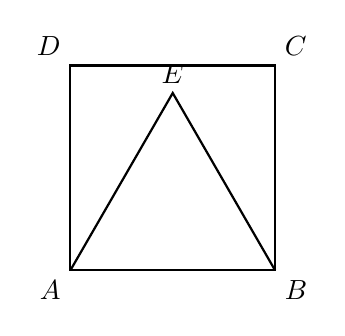
\begin{tikzpicture}[scale=1.3]
		\coordinate (A) at (0,0);
		\coordinate (B) at (2,0);
		\coordinate (C) at (2,2);
		\coordinate (D) at (0,2);
		\coordinate (E) at (1,{sqrt(3)});
		\draw[thick] (A) -- (B) -- (C) -- (D) -- cycle;
		\draw[thick] (A) -- (E) -- (B);
		\node[below left] at (A) {$A$};
		\node[below right] at (B) {$B$};
		\node[above right] at (C) {$C$};
		\node[above left] at (D) {$D$};
		\node[above] at (E) {$E$};
	\end{tikzpicture}
	\end{center}

	% Source: OSK SMA 2010 No. 4 (Isian Singkat)
	% Jawaban: 36 derajat
	\item
	Diberikan segitiga $ABC$, $AB=AC$. Jika titik $P$ di antara $A$ dan $B$ sedemikian rupa sehingga $AP=PC=CB$, maka besarnya sudut $A$ adalah \dots

	% Source: OSK SMP 2010 No. 1 (Isian Singkat)
	% Jawaban: 36 derajat
	\item
	Sebuah $\triangle ABC$ sama kaki dipotong menjadi dua buah segitiga sama kaki (tidak harus kongruen) dengan membagi dua sama besar salah satu sudut alasnya. Ukuran sudut yang terkecil dari segitiga $\triangle ABC$ adalah \dots

	% Source: OSK SMA 2004 No. 17 (Isian Singkat)
	% Jawaban: 5 + 3 akar 5
	\item
	Luas sebuah segitiga siku-siku adalah 5. Panjang sisi miring segitiga ini adalah 5. Maka keliling segitiga tersebut adalah \dots

	% Source: OSK SMA 2012 No. 5 (Isian Singkat)
	% Jawaban: 290
	\item
	Diberikan segitiga siku-siku $ABC$, dengan $AB$ sebagai sisi miringnya. Jika keliling dan luasnya berturut-turut 624 dan 6864, panjang sisi miring segitiga tersebut adalah \dots

	% Source: OSK SMA 2004 No. 8 (Pilihan Ganda)
	% Jawaban: 10
	\item
	Segitiga dengan panjang sisi 6 dan 8 memiliki luas terbesar jika sisi ketiganya memiliki panjang \dots

	% Source: OSK SMP 2018 No. 25 (Pilihan Ganda)
	% Jawaban: akar 3 per 4
	\item
	Diberikan $\Delta ABC$. Jika $AC = AB = 1\text{ cm}$ dan $BC = \sqrt{3}\text{ cm}$, maka luas $\Delta ABC$ adalah \dots\ $\text{cm}^2$.
\end{enumerate}

\section{Kombinatorika}
\begin{enumerate}
	% Source: OSK SMA 2005 No. 15 (Isian Singkat)
	% Jawaban: 12
	\item
	Seorang siswa mempunyai dua celana berwarna biru dan abu-abu, tiga kemeja berwarna putih, merah muda dan kuning, serta dua pasang sepatu berwarna hitam dan coklat. Banyaknya cara siswa tersebut memakai pakaian dan sepatu adalah \dots

	% Source: OSK SMA 2024 No. 2 (Isian Singkat)
	% Jawaban: 1680
	\item
	Diketahui ada 6 pilihan jalan yang dapat digunakan untuk bepergian dari kota A ke kota B dan ada 8 pilihan jalan yang dapat digunakan dari kota B ke kota C. Jika seseorang akan bepergian dari kota A ke kota C melalui kota B dan pulang kembali lagi ke kota A melalui jalan-jalan yang berbeda dari ketika saat pergi, banyaknya cara memilih jalan yang dapat dilalui adalah \dots

	% Source: OSK SMP 2011 No. 19 (Pilihan Ganda)
	% Jawaban: 240
	\item
	Lima orang akan pergi ke pantai menggunakan sebuah mobil berkapasitas 6 tempat duduk. Jika hanya ada dua orang yang bisa menjadi sopir, maka banyaknya cara mengatur tempat duduk mereka di dalam mobil adalah \dots

	% Source: OSK SMP 2010 No. 19 (Pilihan Ganda)
	% Jawaban: 1728
	\item
	Terdapat 3 orang Indonesia, 4 orang Belanda, dan 2 orang Jerman akan duduk dalam bangku yang memanjang. Banyaknya susunan yang terjadi jika duduknya berkelompok menurut kewarganegaraannya adalah \dots

	% Source: OSK SMP 2011 No. 7 (Pilihan Ganda)
	% Jawaban: 3840
	\item
	Lima pasang suami istri akan duduk di 10 kursi secara memanjang. Banyaknya cara mengatur tempat duduk mereka sehingga setiap pasang suami istri duduk berdampingan adalah \dots

	% Source: OSK SMA 2008 No. 3 (Pilihan Ganda)
	% Jawaban: 12
	\item
	Banyaknya susunan huruf B, I, O, L, A sehingga tidak ada dua huruf hidup (\textit{vowel}) yang berturutan adalah \dots

	% Source: OSK SMP 2020 No. 17 (Pilihan Ganda)
	% Jawaban: 90000
	\item
	Diketahui suatu bilangan terdiri dari 6 digit. Jika digit terakhirnya sama dengan digit pertama, maka banyak kemungkinan bilangan tersebut adalah \dots

	% Source: OSK SMP 2021 No. 9 (Pilihan Ganda)
	% Jawaban: 896
	\item
	Sebuah bilangan bulat yang terdiri atas empat digit akan disusun sedemikian sehingga berupa bilangan genap dengan digit pertama (paling kiri) bernilai genap serta tidak ada angka yang berulang. Banyaknya cara menyusun bilangan tersebut adalah \dots
\end{enumerate}

\end{document}
